

% microtype: Tipografía.
% mathpazo: Usa la fuente Palatino.
\documentclass[a4paper, 11pt]{article}
\usepackage[protrusion=true,expansion=true]{microtype}
\usepackage{mathpazo}
\usepackage{booktabs}
\usepackage{multicol}
\usepackage{multirow}

% Indentación de párrafos para Palatino
\setlength{\parindent}{0pt}
  \parskip=8pt
\linespread{1.05} % Change line spacing here, Palatino benefits from a slight increase by default


%%% Castellano.
% noquoting: Permite uso de comillas no españolas.
% lcroman: Permite la enumeración con numerales romanos en minúscula.
% fontenc: Usa la fuente completa para que pueda copiarse correctamente del pdf.
\usepackage[spanish,es-noquoting,es-lcroman]{babel}
\usepackage[utf8]{inputenc}
\usepackage[T1]{fontenc}
\selectlanguage{spanish}


%%% Gráficos
\usepackage{graphicx} % Required for including pictures
\usepackage{wrapfig} % Allows in-line images
\usepackage[usenames,dvipsnames]{color} % Coloring code


%%% Matemáticas
\usepackage{amsmath}
\usepackage[hidelinks]{hyperref}
%%% Código


\usepackage{listings}
\usepackage{graphicx}

%% Listing settings

\usepackage{color}

\definecolor{dkgreen}{rgb}{0,0.6,0}
\definecolor{gray}{rgb}{0.5,0.5,0.5}
\definecolor{mauve}{rgb}{0.58,0,0.82}

\lstset{frame=tb,
  language=Java,
  aboveskip=3mm,
  belowskip=3mm,
  showstringspaces=false,
  columns=flexible,
  basicstyle={\small\ttfamily},
  numbers=none,
  numberstyle=\tiny\color{gray},
  keywordstyle=\color{blue},
  commentstyle=\color{dkgreen},
  stringstyle=\color{mauve},
  breaklines=true,
  breakatwhitespace=true,
  tabsize=3
}



%%% Bibliografía
\makeatletter
\renewcommand\@biblabel[1]{\textbf{#1.}} % Change the square brackets for each bibliography item from '[1]' to '1.'
\renewcommand{\@listI}{\itemsep=0pt} % Reduce the space between items in the itemize and enumerate environments and the bibliography



%----------------------------------------------------------------------------------------
%	TÍTULO
%----------------------------------------------------------------------------------------
% Configuraciones para el título.
% El título no debe editarse aquí.
\renewcommand{\maketitle}{
  \begin{flushright} % Right align
  
  {\LARGE\@title} % Increase the font size of the title
  
  \vspace{50pt} % Some vertical space between the title and author name
  
  {\large\@author} % Author name
  \\\@date % Date
  \vspace{40pt} % Some vertical space between the author block and abstract
  \end{flushright}
}

%% Título
\title{\textbf{Memoria de la práctica 2}\\ % Title
Algorítmica} % Subtitle

\author{\textsc{Fco. Javier Sáez Maldonado}\\ % Author
\textsc{Laura Gómez Garrido}\\
\textsc{Luis Antonio Ortega Andrés}\\
\textsc{Pedro Bonilla Nadal}\\
\textsc{Daniel Pozo Escalona}\vspace{2cm}
\\{\textit{Universidad de Granada}}} % Institution

\date{\today} % Date



%----------------------------------------------------------------------------------------
%	DOCUMENTO
%----------------------------------------------------------------------------------------

\begin{document}

\maketitle % Print the title section


%% Índice
{\parskip=2pt
  \tableofcontents
}
\pagebreak

%%% Inicio del documento


\section{Problema}

Sea un vector $v$ de números de tamaño $n$, todos distintos, de forma que existe un índice $p$ (que no es ni el primero ni el último) tal que a la izquierda de $p$ los números están ordenados de forma creciente y a la derecha de $p$ están ordenados de forma decreciente; es decir
\[
\forall \ i,j \leq p , \ i < j \Rightarrow v[i] < v[j] \quad y \quad \forall \ i,j \geq p, \ i < j \Rightarrow v[i]>v[j]
\]

(de forma que el máximo se encuentra en la posición $p$). Diseñe un algoritmo ``divide y vencerás'' que permita determinar $p$. ¿Cuál es la complejidad del algoritmo? Compárelo con el algoritmo ``obvio'' para realizar esta tarea. Realizar también un estudio empírico e híbrido de la eficiencia de ambos algoritmos.

\section{Solución}

\subsection{El algoritmo obvio}
Lo primero que se nos pedía hacer en la práctica era la implementación de un algoritmo que realice nuestro problema de forma obvia. Como los números no están repetidos y son ascendentes hasta el índice $p$, este $v[p]$ es el máximo del vector. Por tanto, nos bastaría encontrar el índice $t$ tal que:
\[
v[t-1] < v[t] \quad y \quad v[t] > v[t+1]
\]
Así,nuestro algoritmo en\textbf{ \emph{c++} } sería:
\begin{lstlisting}
	int fuerzaBruta(int* v, int n){
		for(int i=1; i < n-1; ++i){
     		if(v[i] > v[i+1])
       	return i;
		}
	}
\end{lstlisting}

Este algoritmo es de orden lineal y queremos mediante la estrategia ``divide y vencerás'' encontrar un algoritmo de orden menor.

\subsection{Divide y vencerás}
Utilizamos ahora la estrategia \textbf{Divide y Vencerás} para crear un algoritmo de orden logarítmico. El algoritmo consiste en ir mirando en la mitad del vector (sea esta mitad la posición $p$) y comparando si los elementos en las posiciones $p-1,p$ y $p+1$ están en orden ascendente, y en cuyo caso realizar de nuevo esta operación sobre el vector que queda a la izquierda de esta posición, o si están en orden descendente, y entonces realizar esta operación sobre el vector que queda a la derecha de esta posición.

Siguiendo este algoritmo escrito en texto, el resultante escrito en el lenguaje \emph{\textbf{c++}} es:
\begin{lstlisting}
int divideYVenceras(int* v, int n){
	int k = n/2;
	if(n==1)
		return 0; //Caso trivial
	
	if(n==2)
		return v[0]>v[1]? 0:1 ; //Entre dos elementos, devuelve el mayor.

	if(v[k] > v[k+1]){

		if(v[k] > v[k-1]) 
			return k;

		//else
		return divideYVenceras(v,k);

	}

	//else
	return k + 1 + divideYVenceras(v+k+1,n-k-1);
}

\end{lstlisting}

Sabemos que nuestro método utiliza la técnica divide y vencerás pues lo que estamos haciendo es dividir el vector en mitades de forma sucesiva.

\subsubsection{La complejidad del algoritmo}
Es un algoritmo de complejidad $log(n)$, dado que para un vector de tamaño n, examinará primero el vector original, después un vector de tamaño $n/2$, después de uno de $n/4$, y así sucesivamente. Por lo tanto para un vector de tamaño $2^n$, hará $n$ examinaciones. Así pués, para uno de tamaño $n$, realizará $log_2(n)$. Por esto, es de orden logarítmico.

\subsubsection{Eficiencia práctica}
Para comparar la eficiencia entre algoritmos, hemos realizado prácticas empíricas. Para el algoritmo lineal realizamos 100 ejecuciones, con $n$ desde $10^6$ hasta $10^8$, con 2 ejecuciones del algoritmo cada ejecución del programa; para el logarítmico las mismas ejecuciones, con $10^5$ ejecuciones del algoritmo cada ejecución del programa, y obtuvimos los resultados adjuntos en la entrega en el fichero ``ejecuciones.dat'', que dan lugar a la siguiente gráfica:

\begin{center}
	\includegraphics[scale=0.22]{grafica1.pdf}
\end{center}

\subsubsection{Eficiencia híbrida}
Una vez sabemos que la eficiencia es de orden logarítmico, realizaremos una aproximación por mínimos cuadrados a una función de tipo $alog(bx) + c$ par el algoritmo divide y vencerás y otra de tipo $ax + b$ para el de orden lineal.

Lo hacemos mediante la herramienta de la GNU: \emph{gnuplot}.
Para ello, primero creamos las funciones:
\begin{lstlisting}
	gnuplot> f(x) = a*x+ b
	gnuplot> g(x) = a*log(x) + b
\end{lstlisting}

Y ahora, los ajustamos a los datos, sabiendo que debido a nuestro formato de salida, en la primera columna están los tamaños del vector, en la segunda el tiempo del algoritmo de fuerza bruta y en la tercera el tiempo del algoritmo divide y vencerás.

\begin{lstlisting}
	gnuplot> fit f(x) "ejecuciones.dat" using 1:2 via a,b
	gnuplot> fit g(x) "ejecuciones.dat" using 1:3 via a,b
\end{lstlisting}

Y por último realizamos el gráfico con GNUPLOT mediante:
\begin{lstlisting}
	gnuplot> plot "ejecuciones.dat" using 1:2 title "Fuerza bruta" , "ejecuciones.dat" using 1:3 title "Divide y vencerás", f(x), g(x)
\end{lstlisting}

Obteniendo el gráfico:
\begin{center}
	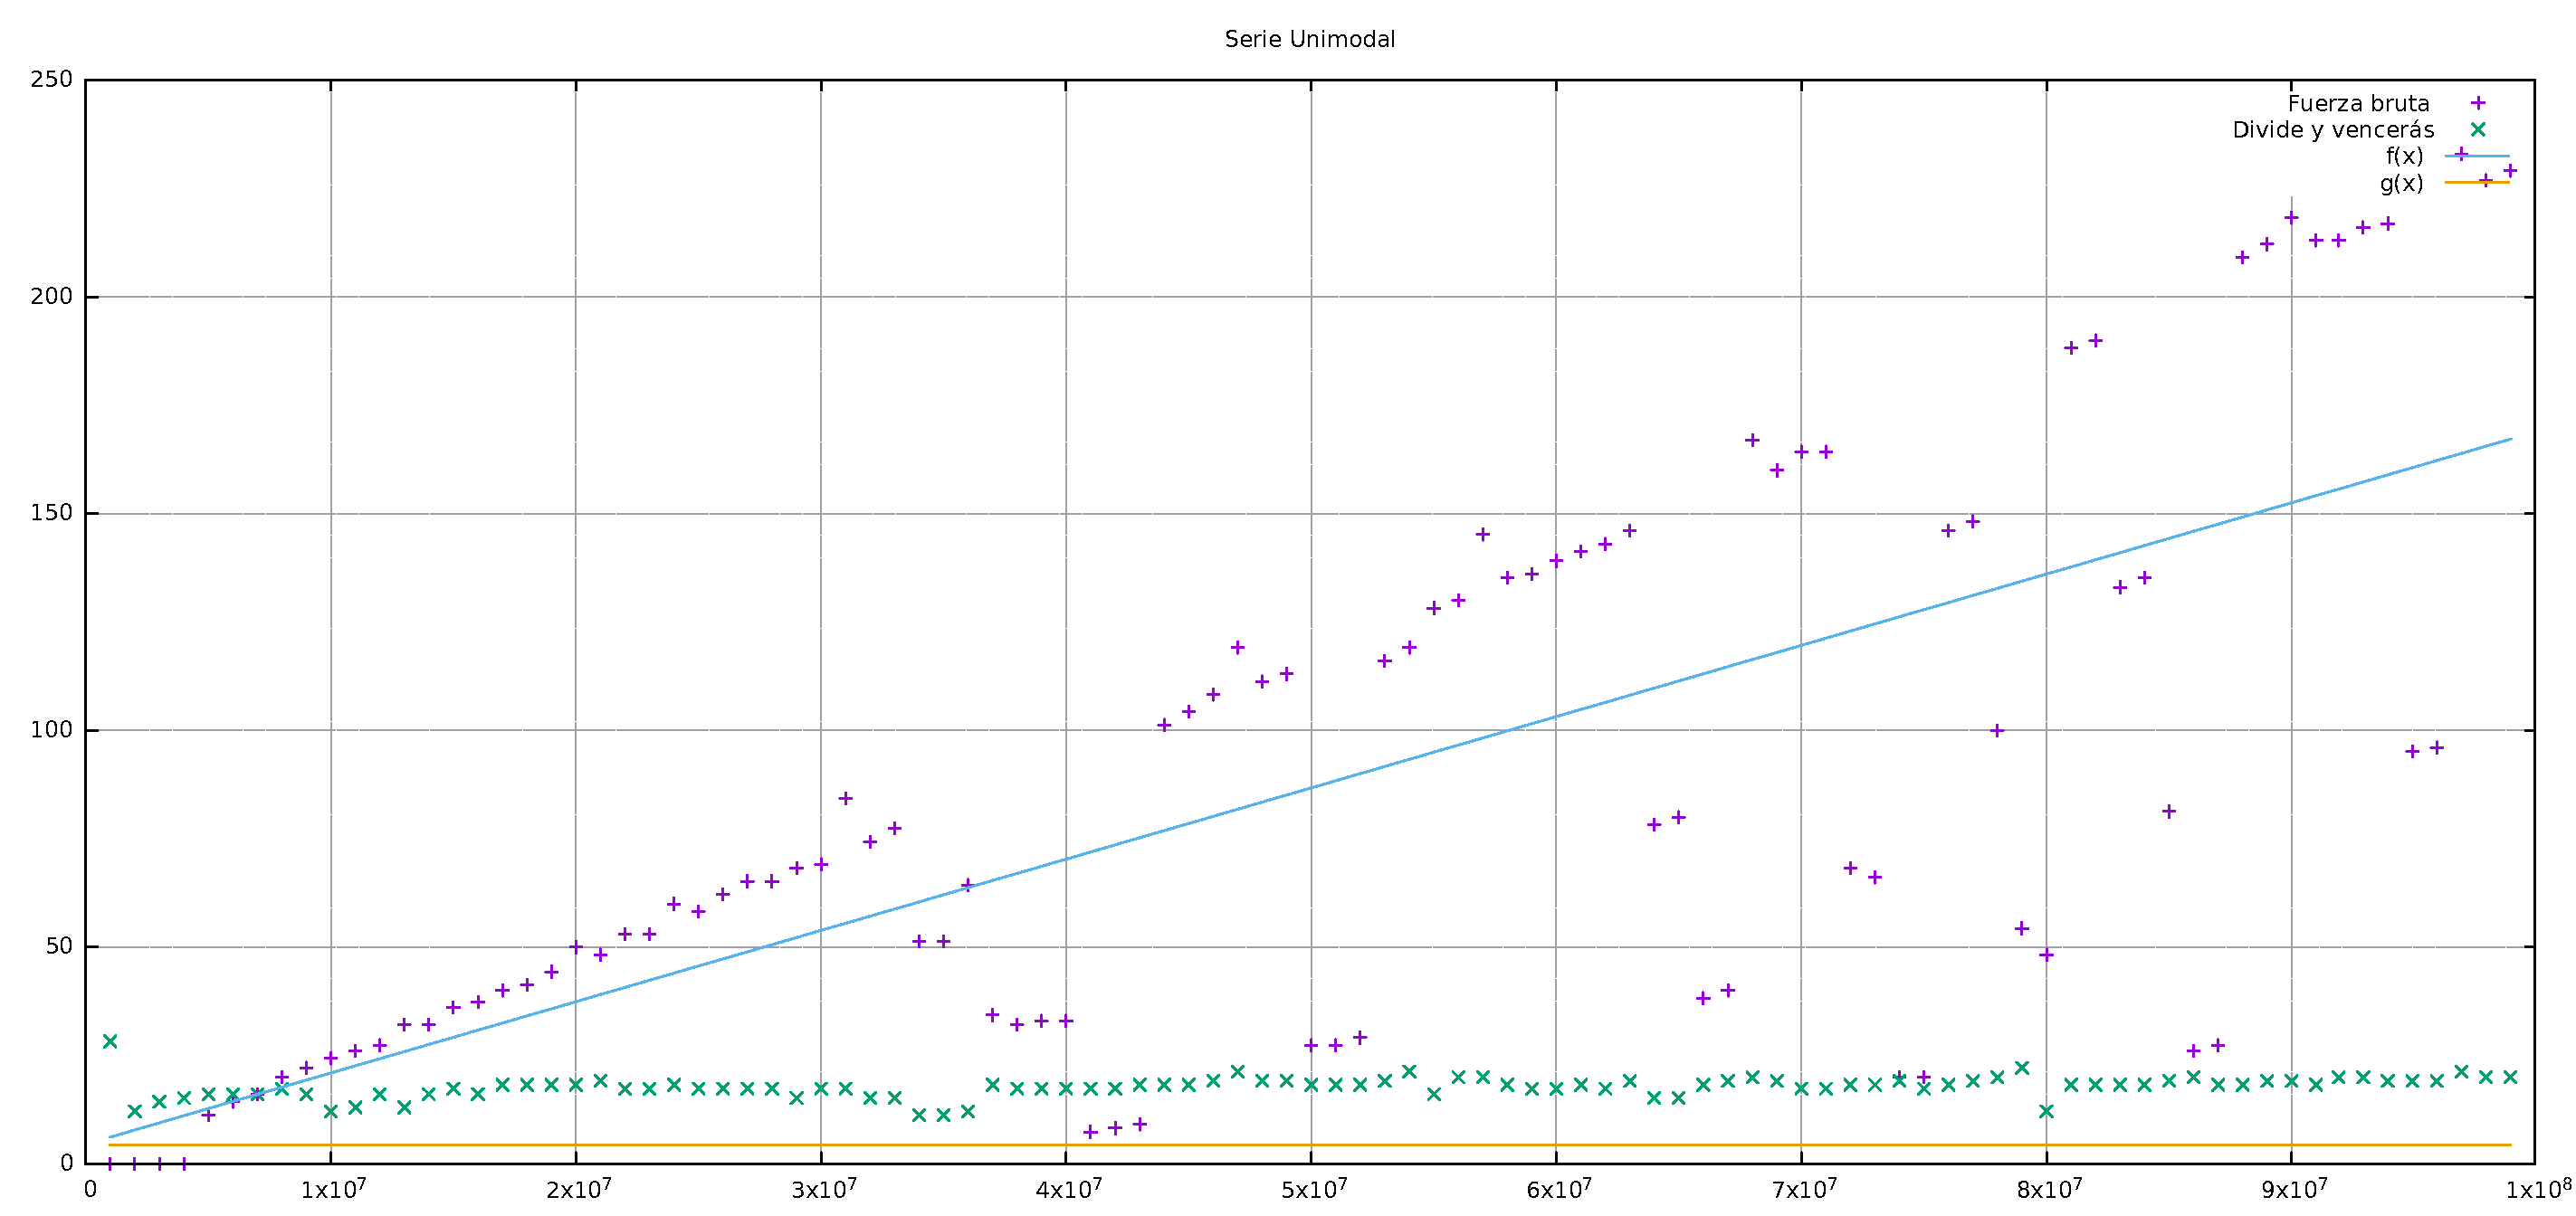
\includegraphics[scale=0.22]{ajuste.pdf}
\end{center}

\subsection{Conclusión}
Como podemos ver en los resultados expuestos, el algoritmo de orden logarítmico o divide y vencerás es claramente mejor a el de orden lineal, lo cual hace clarividente la superioridad de este estilo de algoritmo frente a la fuerza bruta.


\end{document}
